%%%%%%%%%%%%%%%%%%%%%%% file template.tex %%%%%%%%%%%%%%%%%%%%%%%%%
%
% This is a template file for Web of Conferences Journal
%
% Copy it to a new file with a new name and use it as the basis
% for your article
%
%%%%%%%%%%%%%%%%%%%%%%%%%% EDP Science %%%%%%%%%%%%%%%%%%%%%%%%%%%%

%\documentclass{webofc}
% option "twocolumn" for typesetting an article in two columns format (default one column)
 \documentclass[twocolumn]{webofc}
\usepackage{makecell}
\usepackage[varg]{txfonts}   % Web of Conferences font
\usepackage{hyperref}
\usepackage{url}

%% custom commands for thick lines in table
\makeatletter
\newcommand{\thickhlineTwo}{%
    \noalign {\ifnum 0=`}\fi \hrule height 2pt
    \futurelet \reserved@a \@xhline
}
\newcolumntype{"}{@{\hskip\tabcolsep\vrule width 1pt\hskip\tabcolsep}}
\makeatother

\makeatletter
\newcommand{\thickhlineOne}{%
    \noalign {\ifnum 0=`}\fi \hrule height 1pt
    \futurelet \reserved@a \@xhline
}
\makeatother

%%%%%%%%%%%%%%%%%%%%%%%%%%%%%%%%%%%%%%%%%%%%%%%%%%%%%%%%%%%%%%%%%%%%%%%%%%%%%
\hypersetup{colorlinks=true,citecolor=blue,urlcolor=blue,linkcolor=blue}
%%%%%%%%%%%%%%%%%%%%%%%%%%%%%%%%%%%%%%%%%%%%%%%%%%%%%%%%%%%%%%%%%%%%%%%%%%%%%
%
% Put here some packages required or/and some personnal commands
%
%
\begin{document}
%
\title{Overview of the front-end electronics of CMS HGCAL - including readout and powering}
%
% subtitle is optionnal
%
%%%\subtitle{Do you have a subtitle?\\ If so, write it here}


\author{\firstname{Aidan} \lastname{Grummer}\inst{1}\fnsep\thanks{\email{aidan.grummer@cern.ch}} (on behalf of the CMS Collaboration)
        % \firstname{Isabelle} \lastname{Houlbert}\inst{2}\fnsep\thanks{\email{Mail address for second
        %      author if necessary}} \and
        % \firstname{blah} \lastname{Henri}\inst{3}\fnsep\thanks{\email{Mail address for last
        %      author if necessary}}
        % etc.
}

\institute{Fermi National Accelerator Lab.}


\abstract{
The endcap calorimeters of CMS will be upgraded to a single High Granularity Calorimeter (HGCAL) for the HL-LHC, including both silicon sensors and scintillator tiles with on-tile SiPMs as active elements. The readout of the active elements is performed by an ASIC (HGCROC in 130~nm CMOS technology) that measures the amplitude and arrival time of the signals. The amplitude is measured over a large dynamic range to allow calibration with single particles and the measurement of TeV showers. The time of arrival of high-energy showers will be measured with a precision of around 30 ps. A second pair of ``concentrator'' ASICs - ECON-T and ECON-D - takes the data from the HGCROC channels and packages them for transmission via optical links to the off-detector electronics. The ECON-T transmits trigger data at 40 MHz, to form part of the level-1 trigger. The ECON-D transmits concentrated data packets at up to 1 MHz, upon reception of a level-1 trigger signal. In addition to these ASICs HGCAL will use modified versions of common HL-LHC electronics developments, for the power chain and the optical control/readout. The dense nature of the HGCAL provides additional challenges for the electronic boards and cabling. In this proceedings the overall HGCAL front electronics scheme, including the latest performance of the HGCROC and ECON ASICs is presented.
}
%
\maketitle
%
\section{Introduction: HGCal front-end}
\label{intro}
Motivation and technical details of the HGCAL upgrade for operation in HL-LHC may be found in~\cite{CMS:HGCALTDR}.
This proceedings provides an overview of the HGCal frontend. The frontend electronics are used to (1) digitize the signal from the sensors with the HGCal Readout Chip (HGCROC), (2) perform data concentration with the E-link Concentrators (ECON) and (3) to transmit the data using the low power gigabit transceiver (lpGBT) and electrical to optical conversion (VTRX+). Plans for the implementation of the powering and services to the frontend will also be covered.
\section{Section title}
\label{sec-1}
For bibliography
\subsection{Subsection title}
\label{sec-2}
Don't forget to give each section, subsection, subsubsection, and
paragraph a unique label (see Sect.~\ref{sec-1}).

\begin{table*}
\caption{Caption}
\label{tab:req_table}
\centering
    \begin{tabular}{l|l} \hline 
         Parameter & Specification\\ \thickhlineTwo
         Total ionizing dose&  200 Mrad\\ \hline 
         
         \makecell[l]{Tolerance to single event effects (SEE) \\(average detector fluence)} &  Hadron fluence (E $>$ 20 MeV): 1$\times10^{14}$ cm$^{-2}$\\ \thickhlineOne
         
         Charge measurements with large dynamic range &  0.2 fC — 10 pC\\ \hline 
         
         Time resolution &  25 ps\\ \hline
         
         Fit in limited physical space&  $\sim$5 mm gap\\ \hline 
         \makecell[l]{Low power consumption\\(including digitization and concentration on \\DAQ and trigger paths)} & \makecell[l]{$\leq$ 20 mW/ch }\\ \hline 
         
        \makecell[l]{Allow transfer of large data volumes required \\for good trigger and physics performance.} & \makecell[l]{Trigger path: $\sim$60 Tb/s \\DAQ path: $\sim$40 Tb/s}\\\hline
    \end{tabular}
\end{table*}

\begin{figure}[ht]
\centering
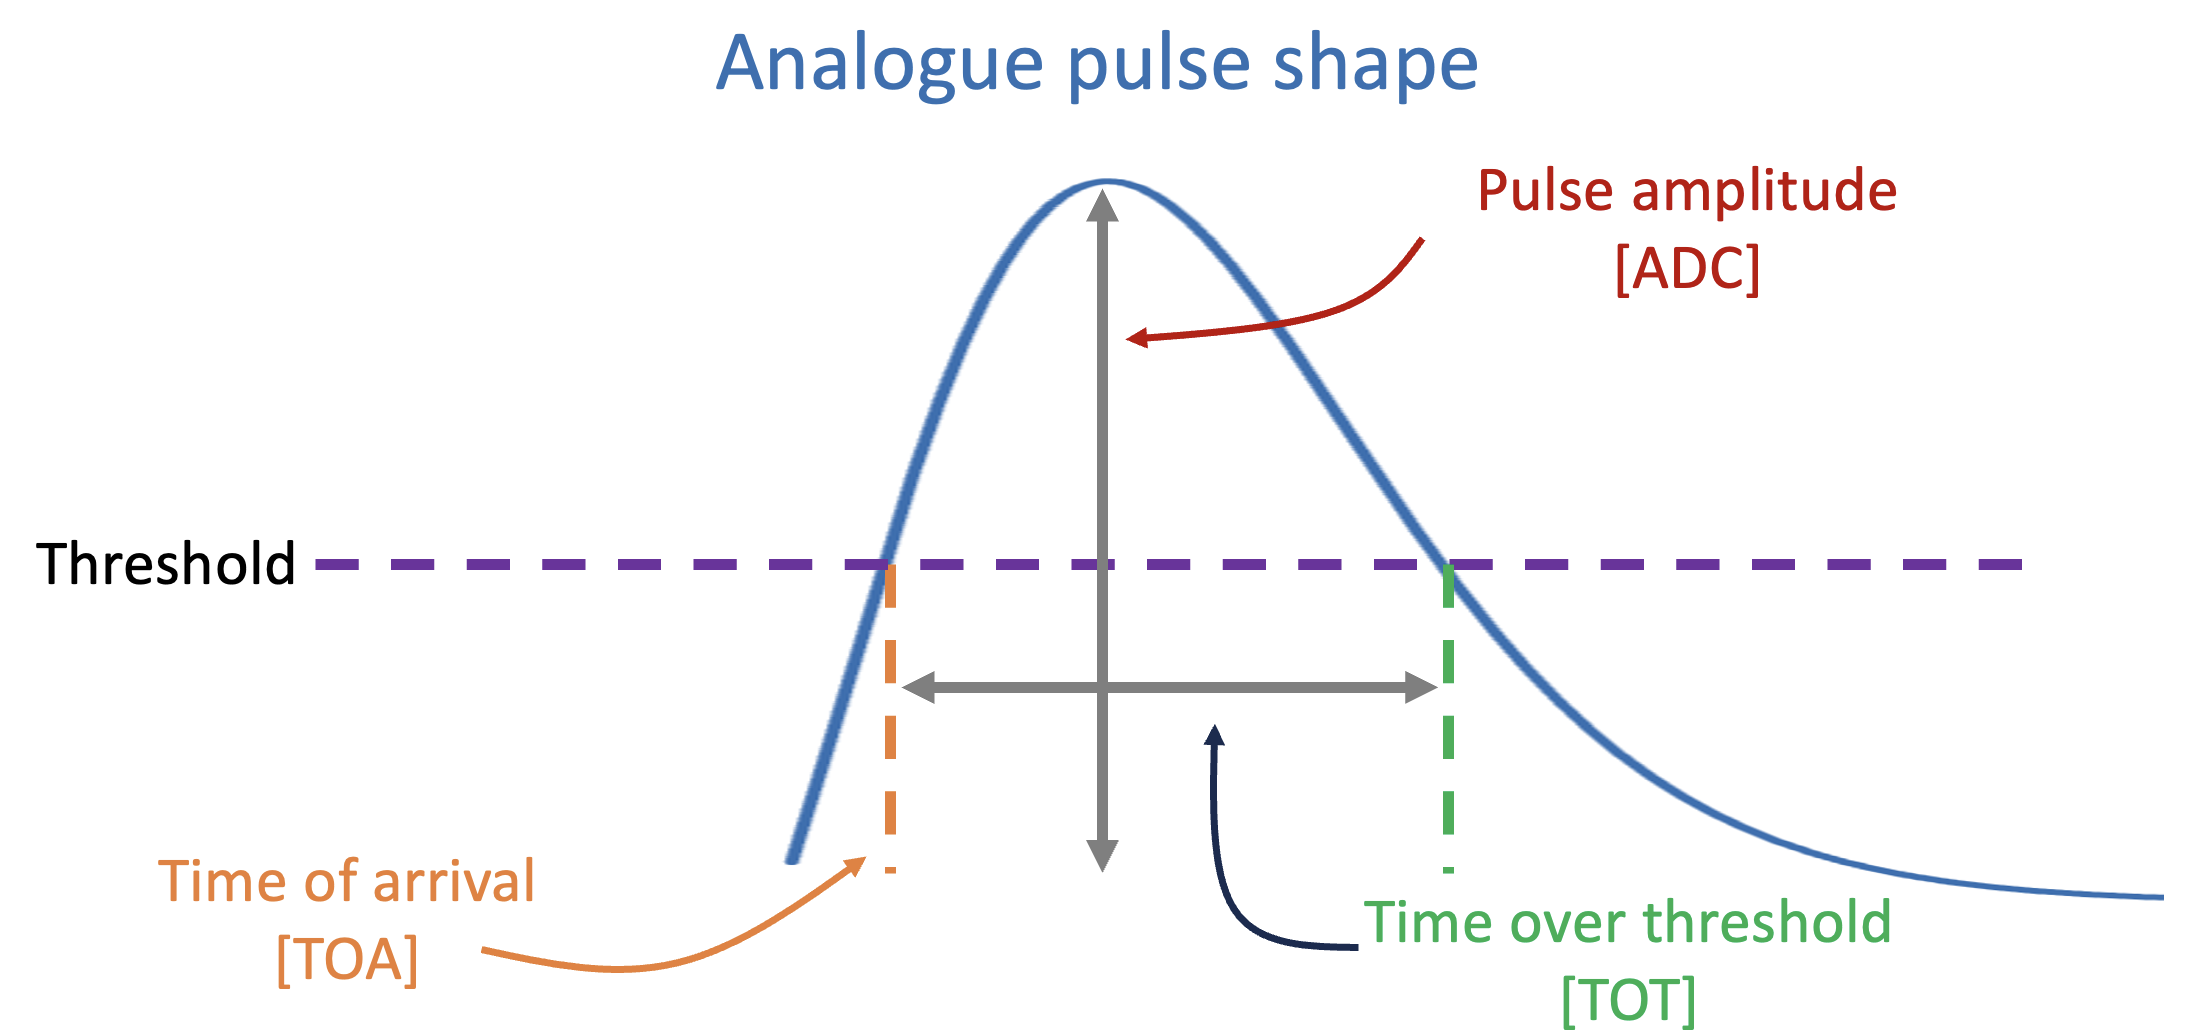
\includegraphics[height=4cm]{figures/PulseShape.png}
\caption{Pulse shape.}
\label{fig:pulse}
\end{figure}

\begin{figure*}[ht]
\centering
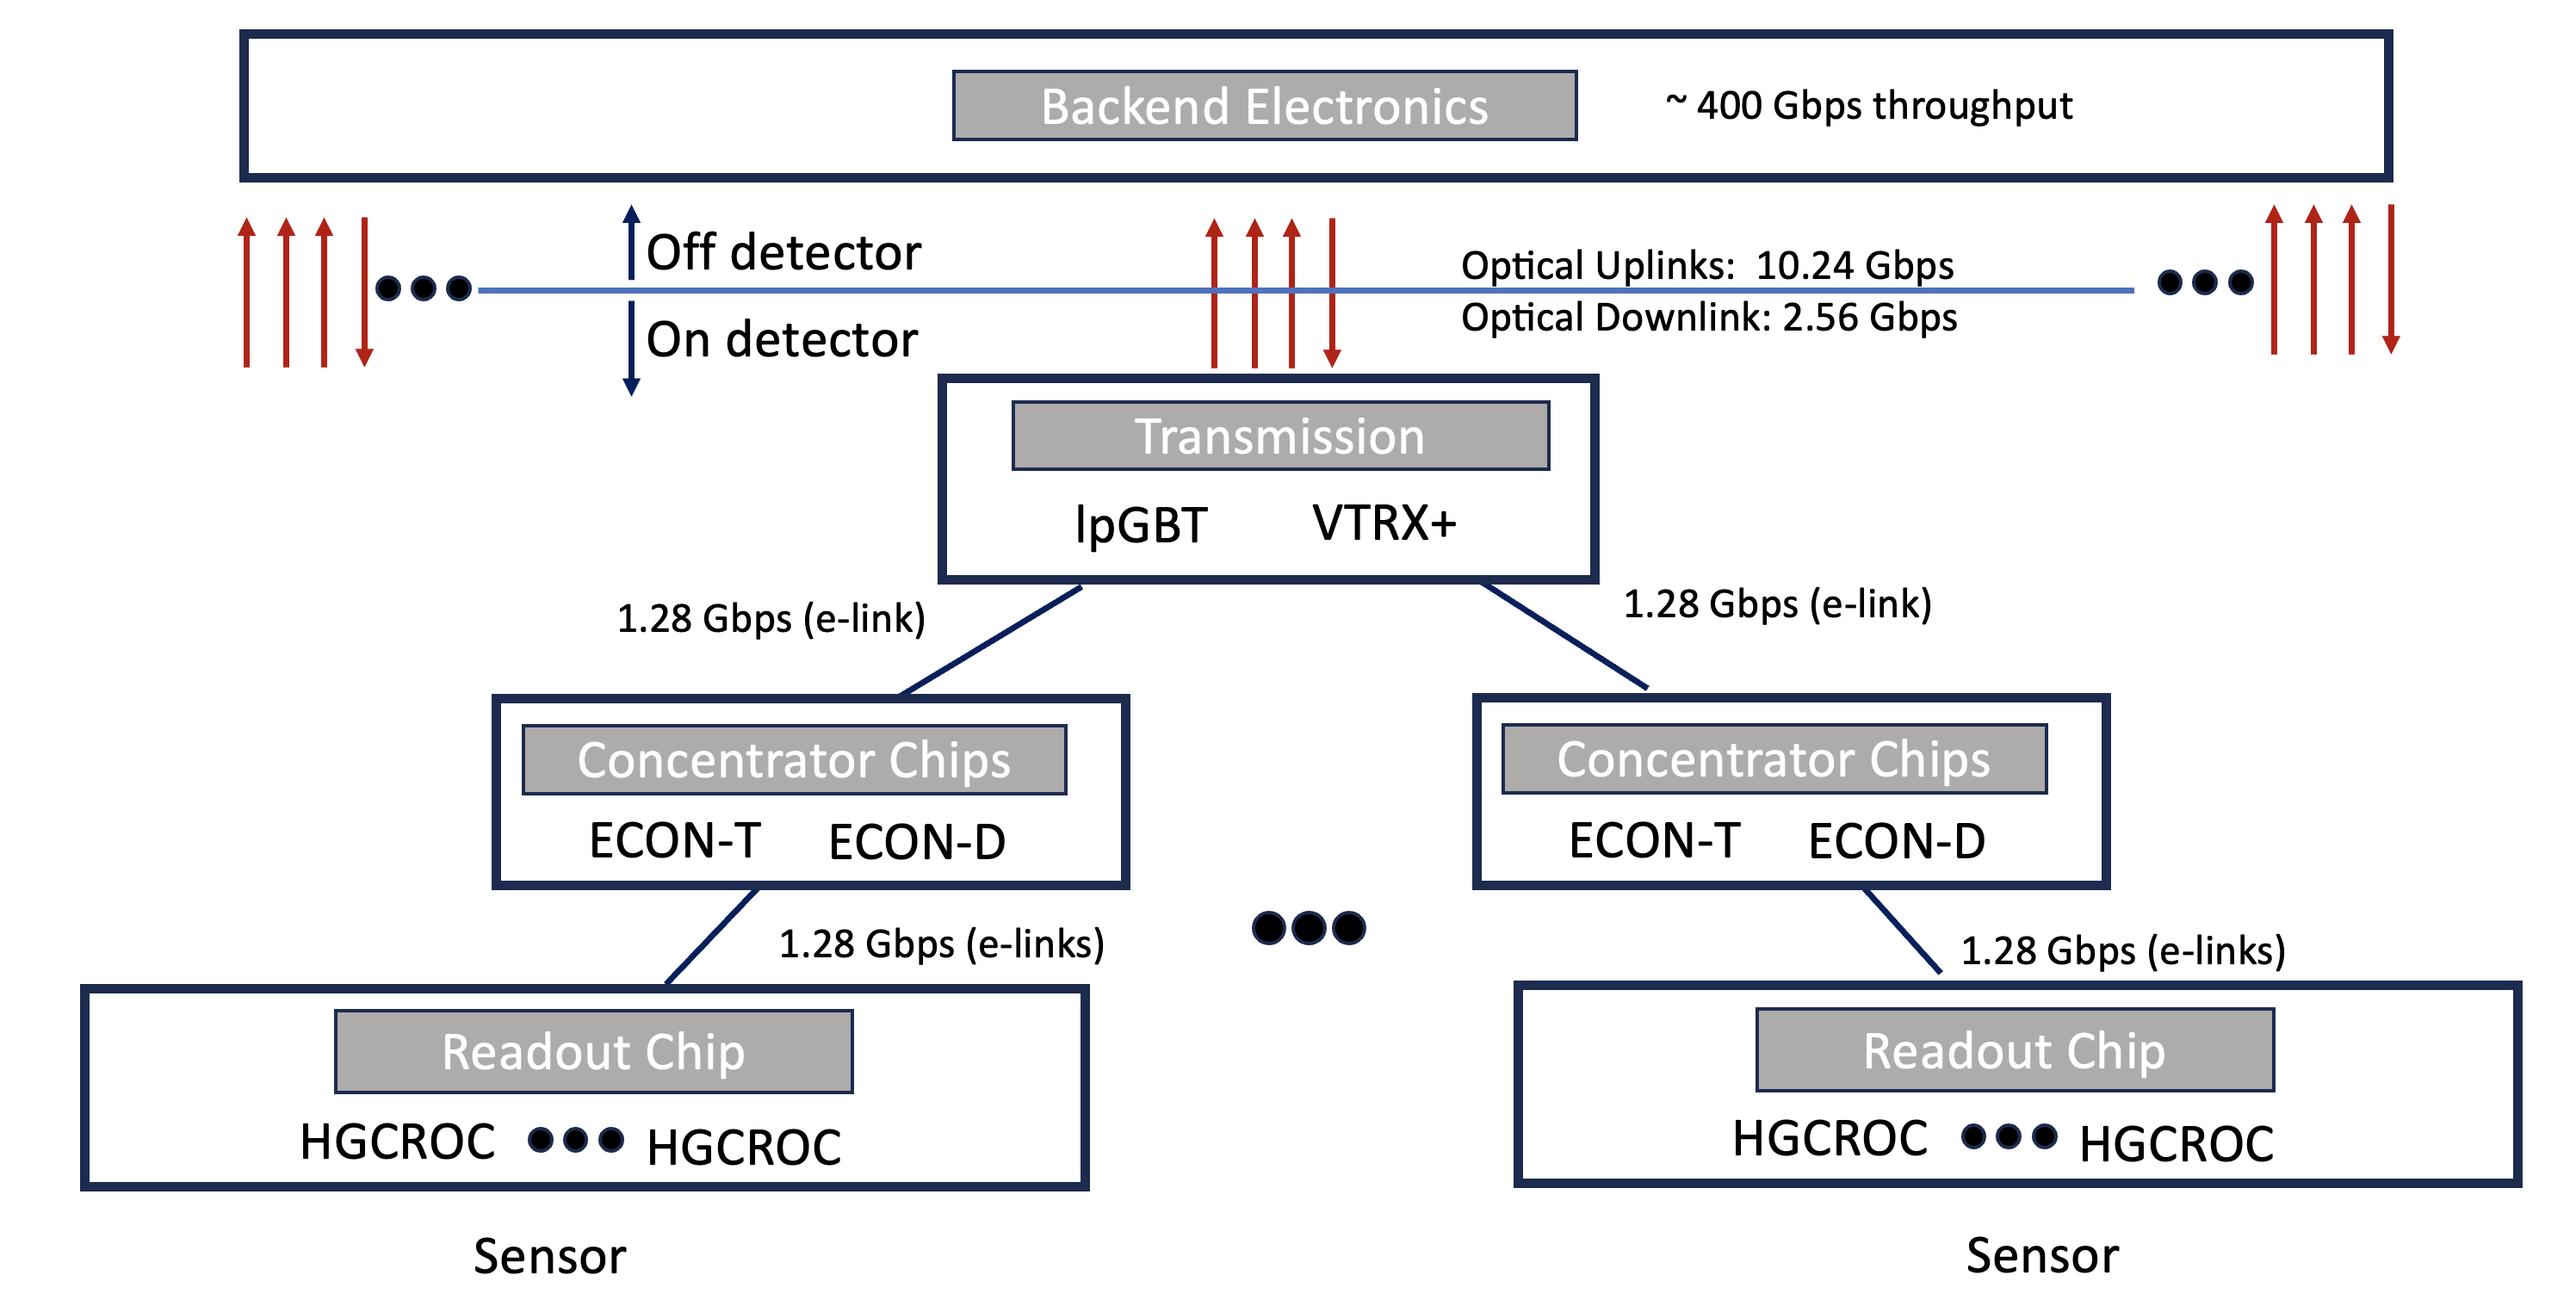
\includegraphics[height=8cm]{figures/ReadoutDiagram.png}
\caption{Front end readout diagram.}
\label{fig:diag}
\end{figure*}
 

\begin{figure*}[ht]
\centering
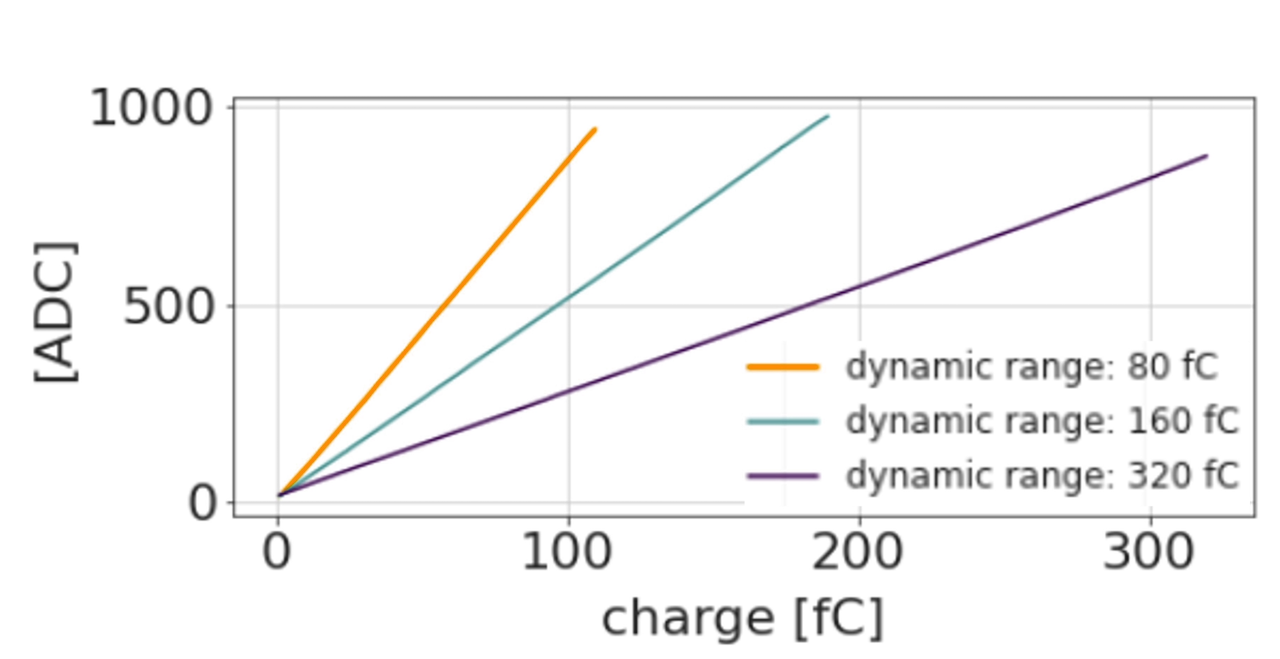
\includegraphics[height=4cm]{figures/roc-ADClinearity.png}
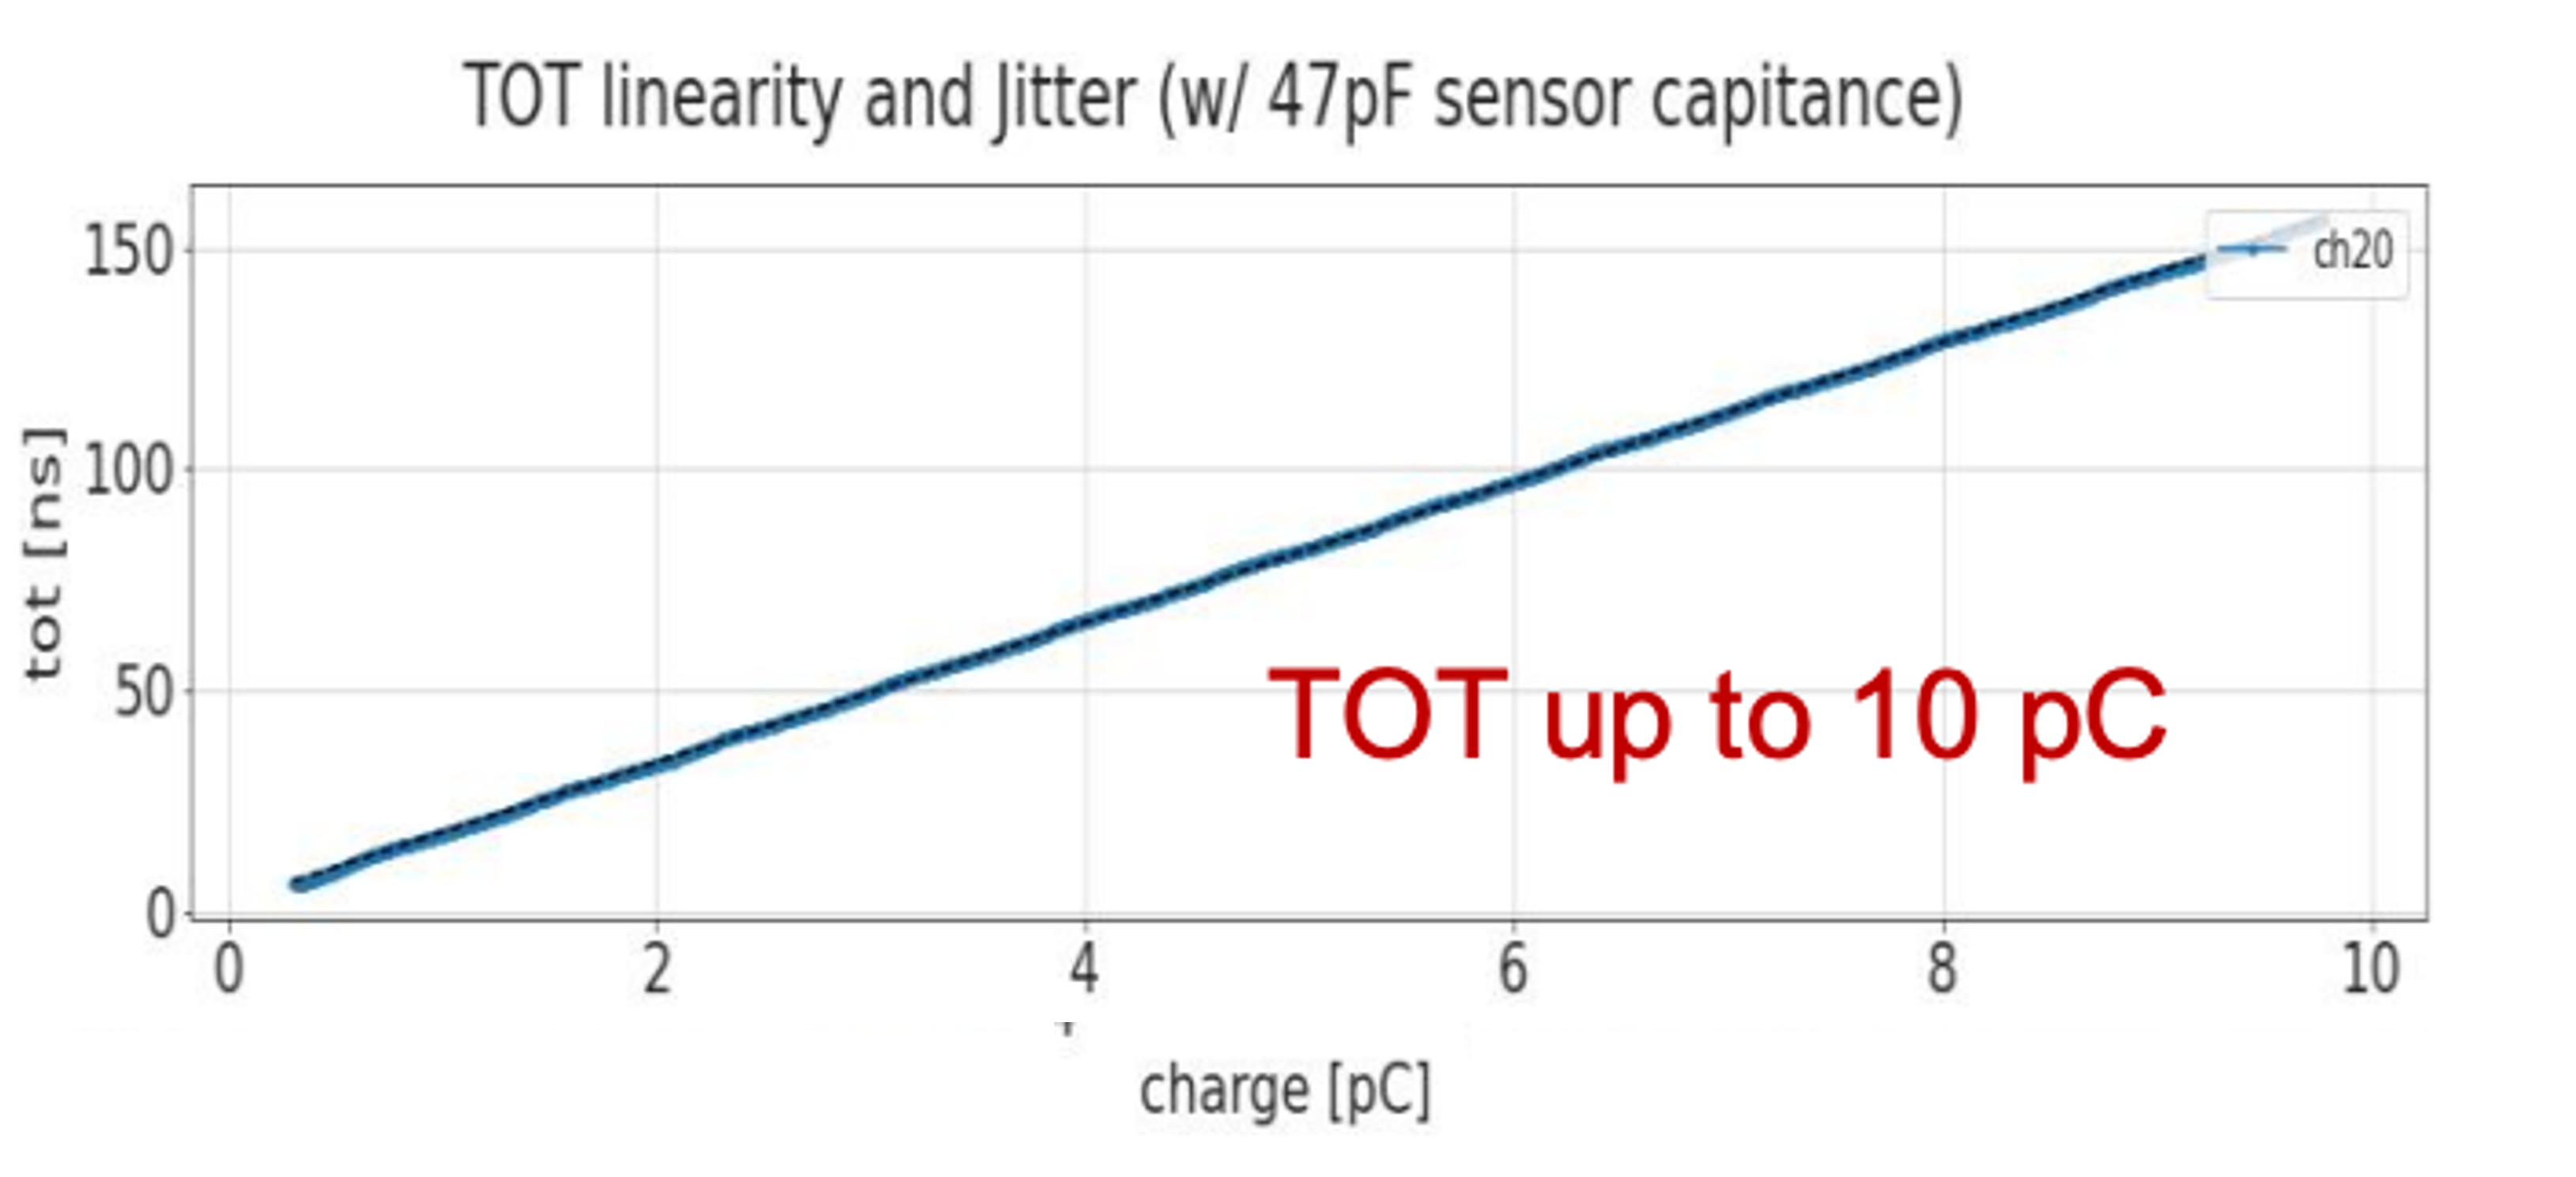
\includegraphics[height=4cm]{figures/roc-TOTlinearity.png}\\
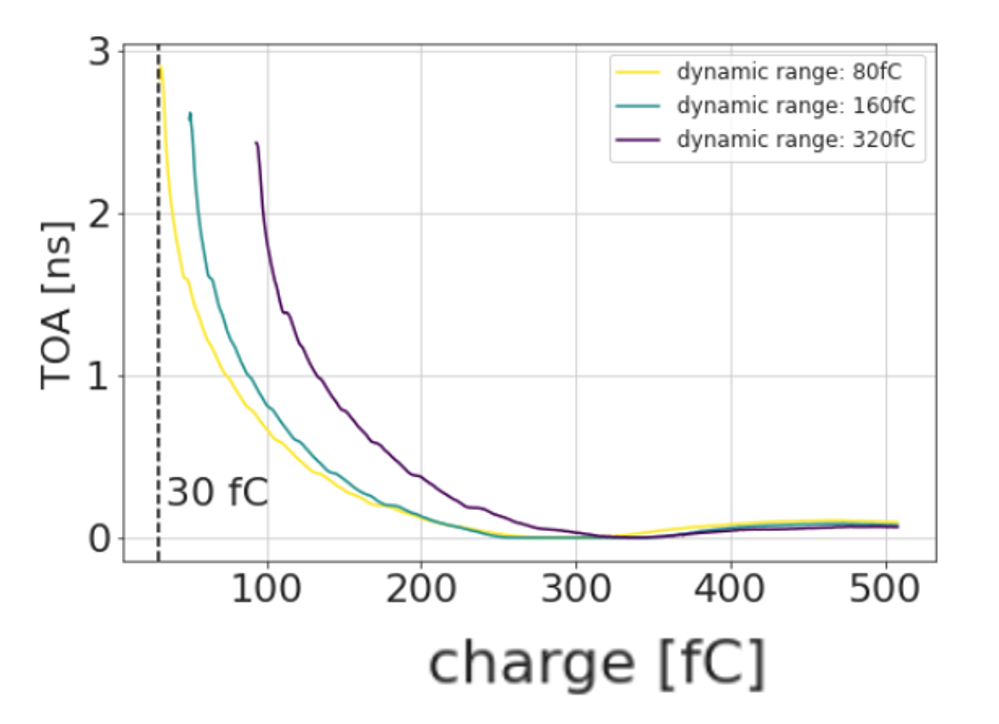
\includegraphics[height=4cm]{figures/roc-toaTimewalk.png}
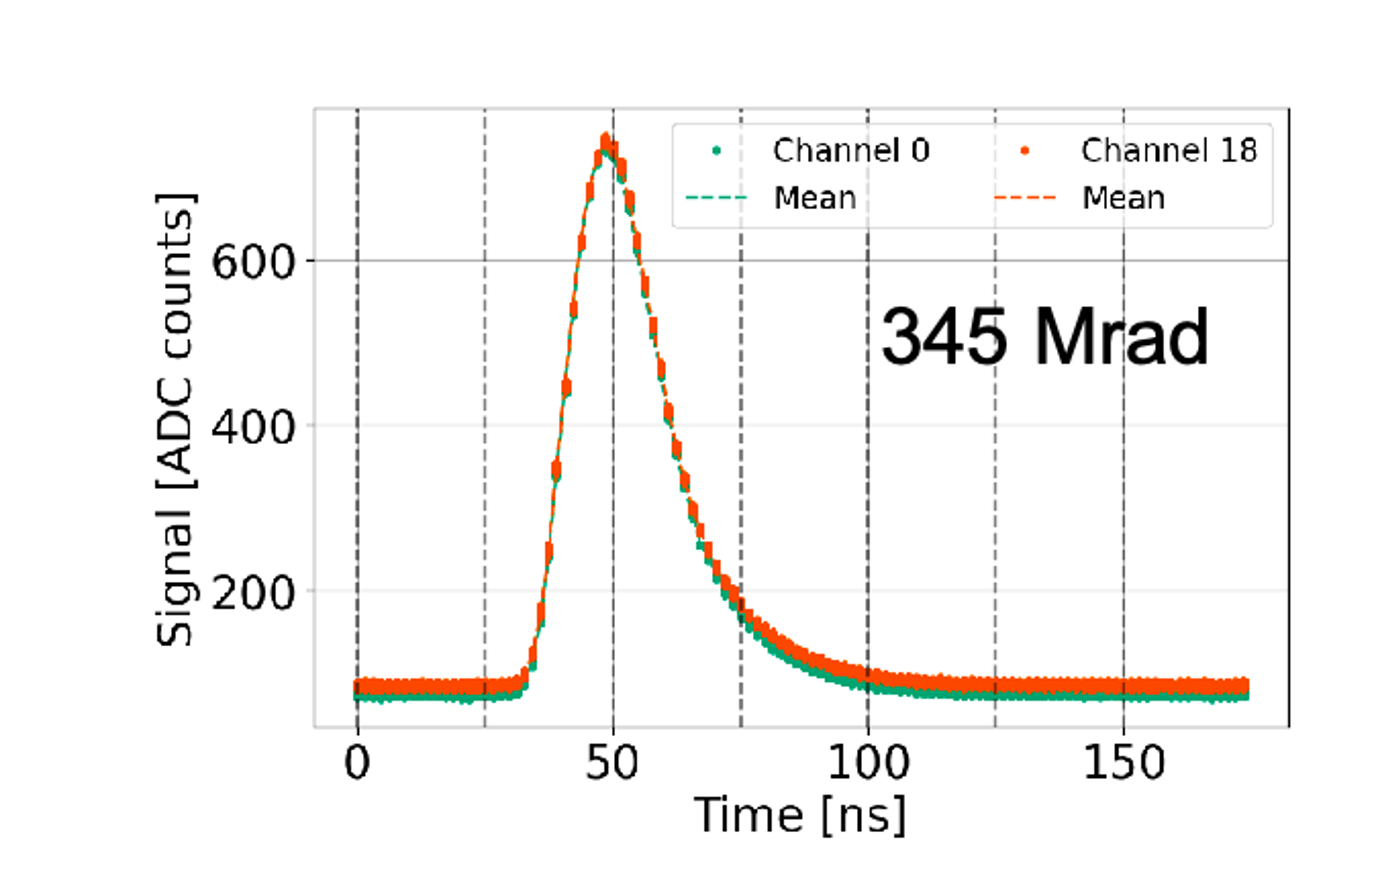
\includegraphics[height=4cm]{figures/roc-ADCirradiation.png}
\caption{(Top left plot) linearity of the HGCROC analogue to digital conversion (ADC) measured for different preamplifier gains is within specification, +/- 0.5\%. (Top right plot) the time over threshold (TOT) linearity is within specification, +/- 0.5\%. (Bottom left plot) time of arrival (TOA) as a function of charge shows a 2.5 ns timewalk. (Bottom right plot) HGCROC ADC signal peak after 345 Mrad TID continues to show stable results.}
\label{fig:roc}
\end{figure*}

\begin{figure*}[ht]
\centering
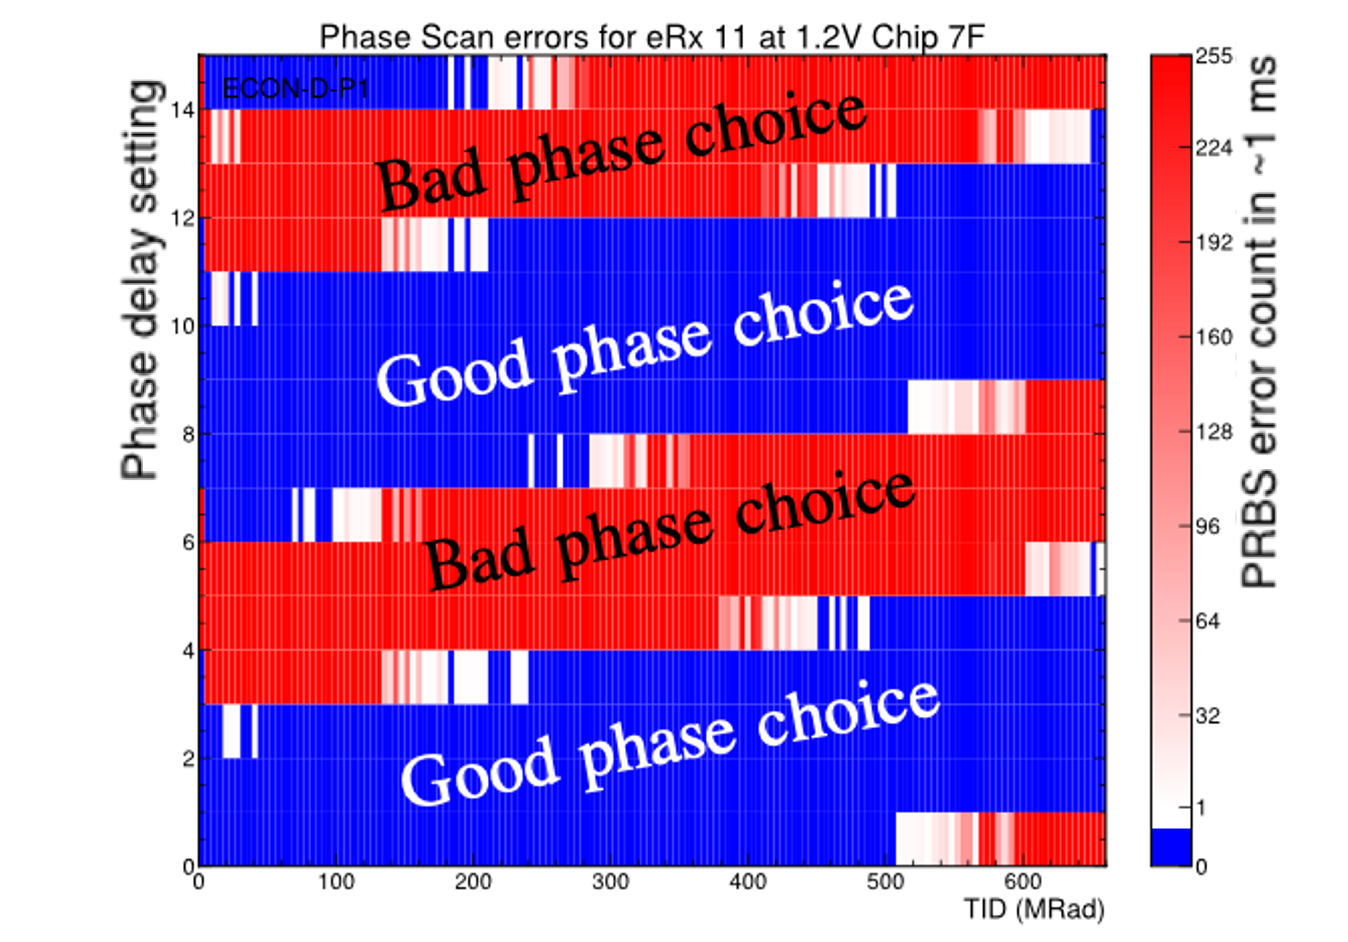
\includegraphics[height=5cm]{figures/econ-phaseTID.png}
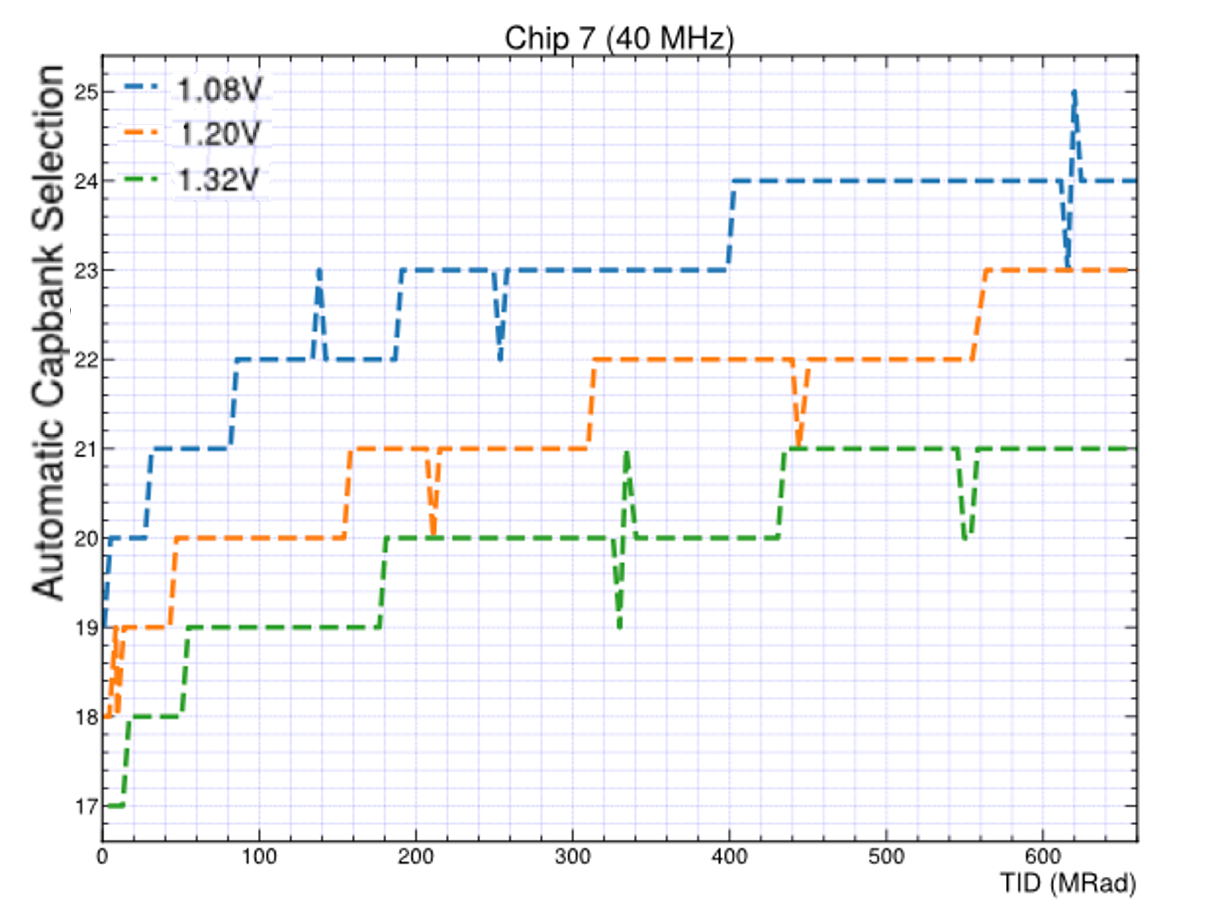
\includegraphics[height=5cm]{figures/econ-capPLLTID.png}
\caption{Total ionizing dose (TID) results for ECON ASICs. (Left plot) evidence of a shift of the good phase window at high TID. For a given choice of phase, the error rate is measured using a pseudo random bit stream; results are as expected. (Right plot) automatic capacitance selection for the phase lock loop (PLL) as a function of TID. Results are shown for the chip operated with different voltages. The capacitance selection results are as expected.}
\label{fig:econ}
\end{figure*}



% For one-column wide figures use syntax of figure~\ref{fig-1}
% \begin{figure}[h]
% % Use the relevant command for your figure-insertion program
% % to insert the figure file.
% \centering
% 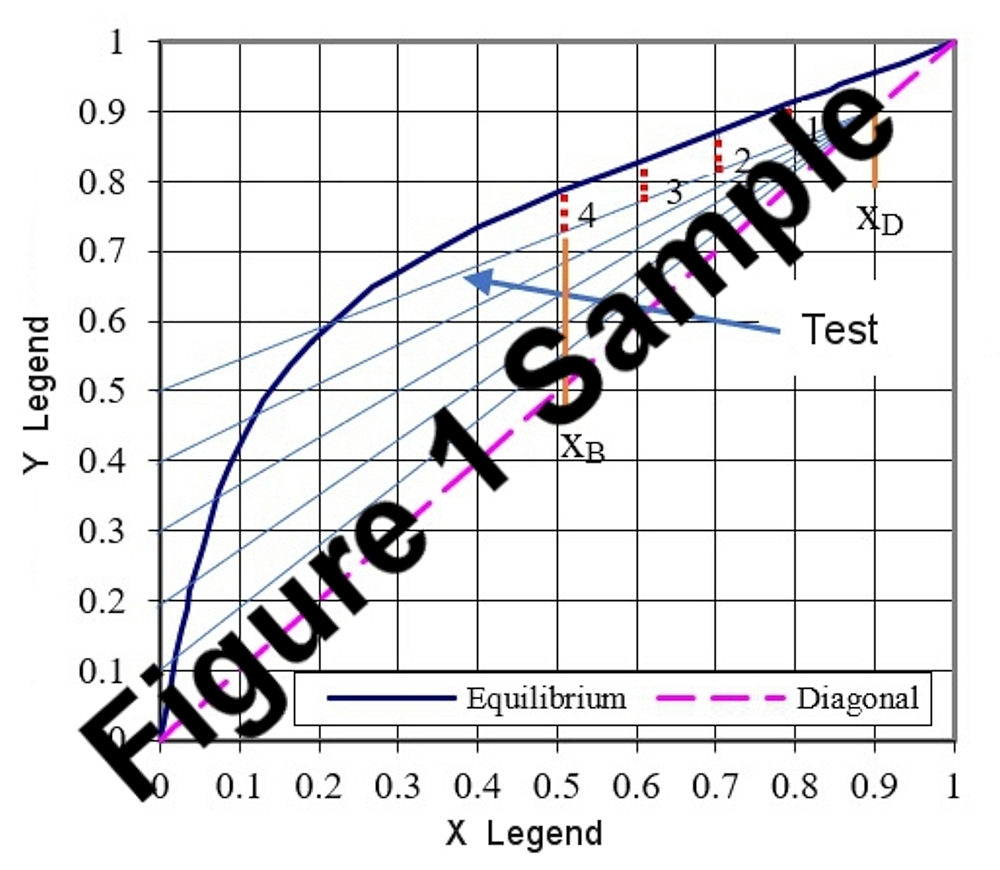
\includegraphics[width=5cm,clip]{fig-1-sample}
% \caption{Please write your figure caption here}
% \label{fig-1}       % Give a unique label
% \end{figure}
% 
% For two-column wide figures use syntax of figure~\ref{fig-2}
% \begin{figure*}
% \centering
% % Use the relevant command for your figure-insertion program
% % to insert the figure file. See example above.
% % If not, use
% \vspace*{1cm}       % Give the correct figure height in cm
% 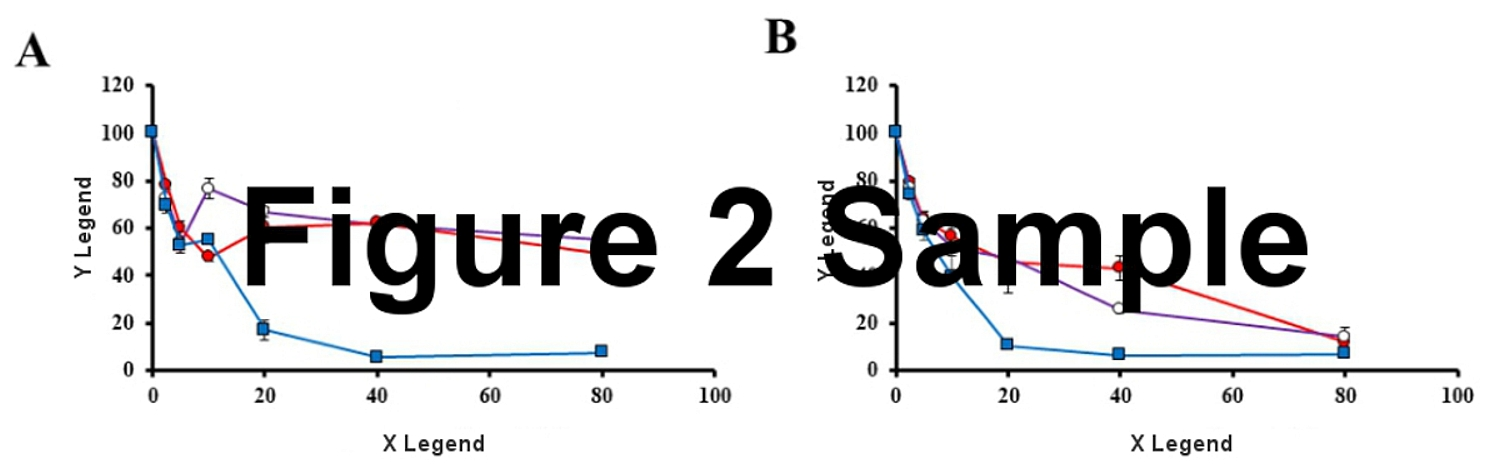
\includegraphics[width=8cm,clip]{fig-2-sample}
% \caption{Please write your figure caption here}
% \label{fig-2}       % Give a unique label
% \end{figure*}
% 
% For tables use syntax in table~\ref{tab-1}.
% \begin{table}
% \centering
% \caption{Please write your table caption here}
% \label{tab-1}       % Give a unique label
% % For LaTeX tables you can use
% \begin{tabular}{lll}
% \hline
% first & second & third  \\\hline
% number & number & number \\
% number & number & number \\
% number & number & number \\\hline
% \end{tabular}
% % Or use
% \vspace*{5cm}  % with the correct table height
% \end{table}
%
% BibTeX or Biber users please use (the style is already called in the class, ensure that the "woc.bst" style is in your local directory)
\bibliography{src/proc.bib} 
%
\end{document}

% end of file template.tex
